% sizes tiny scriptsize footnotesize small normalsize large Large LARGE huge Huge

\documentclass[presentation]{beamer}

\usetheme{JuanLesPins}
\usecolortheme{orchid}
\setbeamertemplate{headline}{}
\setbeamertemplate{navigation symbols}{}

\usepackage{subfig}
\usepackage{graphicx}
\usepackage[english]{babel}
\usepackage[latin1]{inputenc}
\usepackage{color}
\usepackage{listings}
\definecolor{mygreen}{rgb}{0,0.6,0}
\definecolor{mygray}{rgb}{0.5,0.5,0.5}
\definecolor{mymauve}{rgb}{0.58,0,0.82}

\lstset{
  backgroundcolor=\color{white},   % choose the background color; you must add \usepackage{color} or \usepackage{xcolor}; should come as last argument
  basicstyle=\footnotesize\ttfamily, % the size of the fonts that are used for the code
  breakatwhitespace=false,         % sets if automatic breaks should only happen at whitespace
  breaklines=true,                 % sets automatic line breaking
  captionpos=b,                    % sets the caption-position to bottom
  commentstyle=\color{mygreen},    % comment style
  deletekeywords={...},            % if you want to delete keywords from the given language
  escapeinside={\%*}{*)},          % if you want to add LaTeX within your code
  extendedchars=true,              % lets you use non-ASCII characters; for 8-bits encodings only, does not work with UTF-8
  frame=single,	                   % adds a frame around the code
  keepspaces=true,                 % keeps spaces in text, useful for keeping indentation of code (possibly needs columns=flexible)
  keywordstyle=\color{blue},       % keyword style
  morekeywords={*,...},            % if you want to add more keywords to the set
  numbers=none,                    % where to put the line-numbers; possible values are (none, left, right)
  numbersep=5pt,                   % how far the line-numbers are from the code
  numberstyle=\tiny\color{mygray}, % the style that is used for the line-numbers
  rulecolor=\color{black},         % if not set, the frame-color may be changed on line-breaks within not-black text (e.g. comments (green here))
  showspaces=false,                % show spaces everywhere adding particular underscores; it overrides 'showstringspaces'
  showstringspaces=false,          % underline spaces within strings only
  showtabs=false,                  % show tabs within strings adding particular underscores
  stepnumber=2,                    % the step between two line-numbers. If it's 1, each line will be numbered
  stringstyle=\color{mymauve},     % string literal style
  tabsize=2,	                   % sets default tabsize to 2 spaces
  title=\lstname,                  % show the filename of files included with \lstinputlisting; also try caption instead of title
  linewidth=10.7cm,
}

\usepackage{tikz}
\usetikzlibrary{shapes}


% Add any additional packages you use in your presentation
% -----pack
% \usepackage{xxx}
% -----

% Add your custom definitions etc., if required
% -----misc
% \newcommand{\xxx}[1]{[#1]}
% -----




\title{Generational Garbage Collector}
\author{Michal Makson, Rafal Gawel}
\institute{AGH}
\date{}


\begin{document}

\begin{frame}
  \titlepage
\end{frame}

\begin{frame}{Garbage Collector}
Garbage Collector is form of automatic memory management.\\
Its main responsibility is to reclaim memory used to allocate objects that are no longer used.
\end{frame}

\begin{frame}{Weak generational hypothesis}
	Research referred to as Weak Generational Hypothesis
	points two statements:
	\newline
	\begin{itemize}
		\item Most allocated objects die young
		\item Objects tend to live longer past a certain age
	\end{itemize}
\end{frame}

\begin{frame}{Lifetime of Objects}
Illustration presenting tendency of objects lifetime
\newline

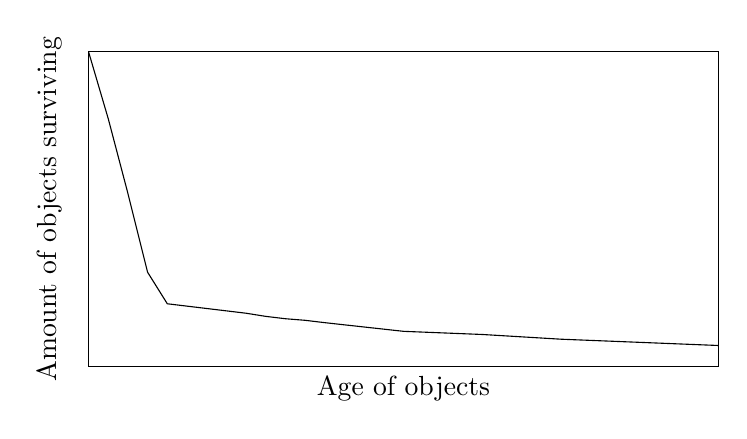
\begin{tikzpicture}
\draw (0, 0) -- (8, 0) -- (8, 4) -- (0, 4) -- (0, 0);
\draw (0, 4) -- (0.25, 3.15) -- (0.5, 2.2) -- (0.75, 1.2)
-- (1, 0.80) -- (1.25, 0.77) -- (1.5, 0.74) -- (1.75, 0.71)
-- (2, 0.68) -- (2.25, 0.64) -- (2.5, 0.61) -- (2.75, 0.59)
-- (3, 0.56) -- (4, 0.45) -- (5, 0.41) -- (6, 0.35) -- (8, 0.27);

\node[bend left, rotate=90] at (-0.5, 2) {Amount of objects surviving};
\node[below] at(4, 0) {Age of objects};
\end{tikzpicture}

\end{frame}

\begin{frame}{Disadvantages of traditional garbage collector}
	Garbage collection is an expensive operation.
	Its execution:
	\newline
	\begin{itemize}
		\item Consumes additional resources
		\item Impacts performance
		\item Stalls program execution
	\end{itemize}
	
\end{frame}

\begin{frame}{Improving performance of Garbage Collector}
	Disadvantages of using garbage collector concern mainly performance. 
	\\Therefore, process optimization was searched.
	\newline
	The solution is Generational Garbage Collector which exploits statements from "Weak generational hypothesis".
\end{frame}


\begin{frame}{Generational Garbage Collection}
	Generational garbage collection algorithms are fastest and most efficient known garbage collection algorithms.
	 The main assumptions are that:
	 \newline
	 \begin{itemize}
	 	\item Heap memory is divided into older and newer objects areas
	 	\item Most of the time garbage collection process runs only on newer objects area
	 	\item Collection of older objects is processed only when necessary
	 \end{itemize}
\end{frame}

\begin{frame}{Memory division - program data area}
	Except older and newer objects memory blocks, there is also a third memory block - program data area.
	\newline
	This fact is exploited to make garbage collector collect only the fresh objects.
\end{frame}

\begin{frame}{Minor Collection}
	To activate garbage collection process only on newer objects a simple trick is used.
	\\
	The trick is to consider older objects memory blocks as part of program data area.
	\\
	By doing so, we avoid garbage collector collecting from older objects area.
\end{frame}

\begin{frame}{Root set - pointers to objects}
	The vast majority of pointers to new object is located in newer objects area.
	\\
	To improve garbage collection process even further this fact is utilized.
	\\
	Some algorithms store pointers to newer objects located in older objects area to avoid scanning for them during garbage collection process.
\end{frame}

\begin{frame}{Before a generational Minor Collection}
	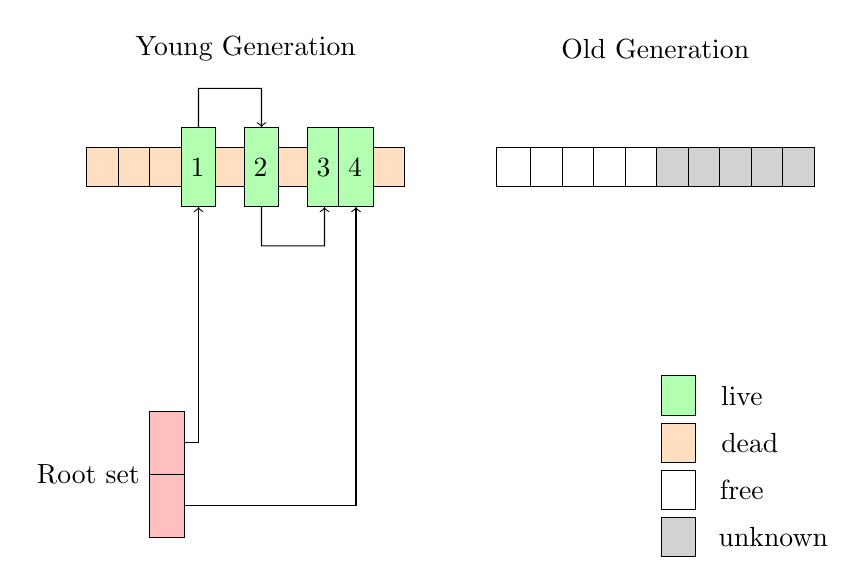
\begin{tikzpicture}
	\node[xshift=2cm] {Young Generation};
	\node[yshift=-1.5cm,xshift=0.2cm,draw, rectangle,fill=orange!25,text width=0.2cm, minimum height=0.5cm] {};
	\node[yshift=-1.5cm,xshift=0.6cm,draw, rectangle,fill=orange!25,text width=0.2cm, minimum height=0.5cm] {};
	\node[yshift=-1.5cm,xshift=1cm,draw, rectangle,fill=orange!25,text width=0.2cm, minimum height=0.5cm] {};
	\node[yshift=-1.5cm,xshift=1.8cm,draw, rectangle,fill=orange!25,text width=0.2cm, minimum height=0.5cm] (3) {};
	\node[yshift=-1.5cm,xshift=2.6cm,draw, rectangle,fill=orange!25,text width=0.2cm, minimum height=0.5cm] {};
	\node[yshift=-1.5cm,xshift=3.8cm,draw, rectangle,fill=orange!25,text width=0.2cm, minimum height=0.5cm] {};
	\node[yshift=-1.5cm,xshift=1.4cm,draw, rectangle,fill=green!30,text width=0.2cm, minimum height=1cm] (1) {1};
	\node[yshift=-1.5cm,xshift=2.2cm,draw, rectangle,fill=green!30,text width=0.2cm, minimum height=1cm] (2) {2};
	\node[yshift=-1.5cm,xshift=3cm,draw, rectangle,fill=green!30,text width=0.2cm, minimum height=1cm] (3) {3};
	\node[yshift=-1.5cm,xshift=3.4cm,draw, rectangle,fill=green!30,text width=0.2cm, minimum height=1cm] (4) {4};
	
	
	\node[xshift=7.2cm] () {Old Generation};
	\node[yshift=-1.5cm,xshift=9cm,draw, rectangle,fill=gray!35,text width=0.2cm, minimum height=0.5cm] {};
	\node[yshift=-1.5cm,xshift=8.6cm,draw, rectangle,fill=gray!35,text width=0.2cm, minimum height=0.5cm] {};
	\node[yshift=-1.5cm,xshift=8.2cm,draw, rectangle,fill=gray!35,text width=0.2cm, minimum height=0.5cm] {};
	\node[yshift=-1.5cm,xshift=7.8cm,draw, rectangle,fill=gray!35,text width=0.2cm, minimum height=0.5cm] {};
	\node[yshift=-1.5cm,xshift=7.4cm,draw, rectangle,fill=gray!35,text width=0.2cm, minimum height=0.5cm] {};
	\node[yshift=-1.5cm,xshift=7cm,draw, rectangle,fill=white,text width=0.2cm, minimum height=0.5cm] {};
	\node[yshift=-1.5cm,xshift=6.6cm,draw, rectangle,fill=white,text width=0.2cm, minimum height=0.5cm] {};
	\node[yshift=-1.5cm,xshift=6.2cm,draw, rectangle,fill=white,text width=0.2cm, minimum height=0.5cm] {};
	\node[yshift=-1.5cm,xshift=5.8cm,draw, rectangle,fill=white,text width=0.2cm, minimum height=0.5cm] {};
	\node[yshift=-1.5cm,xshift=5.4cm,draw, rectangle,fill=white,text width=0.2cm, minimum height=0.5cm] {};
	
	\node[yshift=-4.4cm,xshift=8.3cm] {live};
	\node[yshift=-4.4cm,xshift=7.5cm,draw, rectangle,fill=green!30,text width=0.2cm, minimum height=0.5cm] {};
	\node[yshift=-5cm,xshift=8.4cm] {dead};
	\node[yshift=-5cm,xshift=7.5cm,draw, rectangle,fill=orange!25,text width=0.2cm, minimum height=0.5cm] {};
	\node[yshift=-5.6cm,xshift=8.3cm] {free};
	\node[yshift=-5.6cm,xshift=7.5cm,draw, rectangle,fill=white,text width=0.2cm, minimum height=0.5cm] {};
	\node[yshift=-6.2cm,xshift=8.7cm] {unknown};
	\node[yshift=-6.2cm,xshift=7.5cm,draw, rectangle,fill=gray!35,text width=0.2cm, minimum height=0.5cm] {};
	
	\node[yshift=-5.4cm] {Root set};
	\node[xshift=1cm,yshift=-5cm,draw, rectangle,fill=red!25,text width=0.2cm, minimum height=0.8cm] (R1) {};
	\node[xshift=1cm,yshift=-5.8cm,draw, rectangle,fill=red!25,text width=0.2cm, minimum height=0.8cm] (R2) {};
	\draw[->, to path={-| (\tikztotarget)}] (R1) edge (1);
	\draw[->, to path={-| (\tikztotarget)}] (R2) edge (4);
	\draw[->] (1) -- (1.4,-0.5) -- (2.2,-0.5) -> (2);
	\draw[->] (2) -- (2.2,-2.5) -- (3,-2.5) -> (3);
	\end{tikzpicture}
\end{frame}

\begin{frame}{After a generational Minor Collection}
	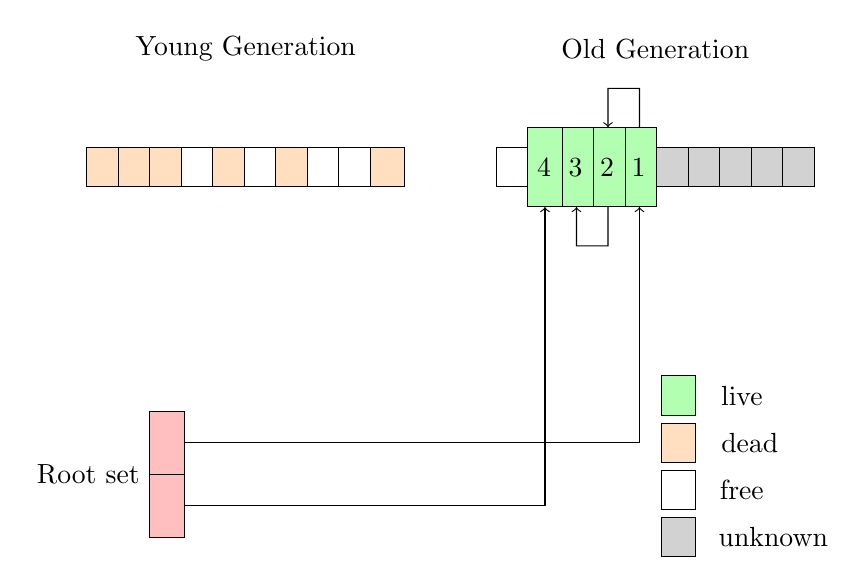
\begin{tikzpicture}
	\node[xshift=2cm] {Young Generation};
	\node[yshift=-1.5cm,xshift=0.2cm,draw, rectangle,fill=orange!25,text width=0.2cm, minimum height=0.5cm] {};
	\node[yshift=-1.5cm,xshift=0.6cm,draw, rectangle,fill=orange!25,text width=0.2cm, minimum height=0.5cm] {};
	\node[yshift=-1.5cm,xshift=1cm,draw, rectangle,fill=orange!25,text width=0.2cm, minimum height=0.5cm] {};
	\node[yshift=-1.5cm,xshift=1.4cm,draw, rectangle,fill=white,text width=0.2cm, minimum height=0.5cm] {};
	\node[yshift=-1.5cm,xshift=1.8cm,draw, rectangle,fill=orange!25,text width=0.2cm, minimum height=0.5cm] (3) {};
	\node[yshift=-1.5cm,xshift=2.2cm,draw, rectangle,fill=white,text width=0.2cm, minimum height=0.5cm] {};
	\node[yshift=-1.5cm,xshift=2.6cm,draw, rectangle,fill=orange!25,text width=0.2cm, minimum height=0.5cm] {};
	\node[yshift=-1.5cm,xshift=3cm,draw, rectangle,fill=white,text width=0.2cm, minimum height=0.5cm] {};
	\node[yshift=-1.5cm,xshift=3.4cm,draw, rectangle,fill=white,text width=0.2cm, minimum height=0.5cm] {};
	\node[yshift=-1.5cm,xshift=3.8cm,draw, rectangle,fill=orange!25,text width=0.2cm, minimum height=0.5cm] {};
	
	
	
	
	
	\node[xshift=7.2cm] () {Old Generation};
	\node[yshift=-1.5cm,xshift=9cm,draw, rectangle,fill=gray!35,text width=0.2cm, minimum height=0.5cm] {};
	\node[yshift=-1.5cm,xshift=8.6cm,draw, rectangle,fill=gray!35,text width=0.2cm, minimum height=0.5cm] {};
	\node[yshift=-1.5cm,xshift=8.2cm,draw, rectangle,fill=gray!35,text width=0.2cm, minimum height=0.5cm] {};
	\node[yshift=-1.5cm,xshift=7.8cm,draw, rectangle,fill=gray!35,text width=0.2cm, minimum height=0.5cm] {};
	\node[yshift=-1.5cm,xshift=7.4cm,draw, rectangle,fill=gray!35,text width=0.2cm, minimum height=0.5cm] {};
	\node[yshift=-1.5cm,xshift=5.4cm,draw, rectangle,fill=white,text width=0.2cm, minimum height=0.5cm] {};
	\node[yshift=-1.5cm,xshift=7cm,draw, rectangle,fill=green!30,text width=0.2cm, minimum height=1cm] (1) {1};
	\node[yshift=-1.5cm,xshift=6.6cm,draw, rectangle,fill=green!30,text width=0.2cm, minimum height=1cm] (2) {2};
	\node[yshift=-1.5cm,xshift=6.2cm,draw, rectangle,fill=green!30,text width=0.2cm, minimum height=1cm] (3) {3};
	\node[yshift=-1.5cm,xshift=5.8cm,draw, rectangle,fill=green!30,text width=0.2cm, minimum height=1cm] (4) {4};
	
	\node[yshift=-4.4cm,xshift=8.3cm] {live};
	\node[yshift=-4.4cm,xshift=7.5cm,draw, rectangle,fill=green!30,text width=0.2cm, minimum height=0.5cm] {};
	\node[yshift=-5cm,xshift=8.4cm] {dead};
	\node[yshift=-5cm,xshift=7.5cm,draw, rectangle,fill=orange!25,text width=0.2cm, minimum height=0.5cm] {};
	\node[yshift=-5.6cm,xshift=8.3cm] {free};
	\node[yshift=-5.6cm,xshift=7.5cm,draw, rectangle,fill=white,text width=0.2cm, minimum height=0.5cm] {};
	\node[yshift=-6.2cm,xshift=8.7cm] {unknown};
	\node[yshift=-6.2cm,xshift=7.5cm,draw, rectangle,fill=gray!35,text width=0.2cm, minimum height=0.5cm] {};
	
	\node[yshift=-5.4cm] {Root set};
	\node[xshift=1cm,yshift=-5cm,draw, rectangle,fill=red!25,text width=0.2cm, minimum height=0.8cm] (R1) {};
	\node[xshift=1cm,yshift=-5.8cm,draw, rectangle,fill=red!25,text width=0.2cm, minimum height=0.8cm] (R2) {};
	\draw[->, to path={-| (\tikztotarget)}] (R1) edge (1);
	\draw[->, to path={-| (\tikztotarget)}] (R2) edge (4);
	\draw[->] (1) -- (7,-0.5) -- (6.6,-0.5) -> (2);
	\draw[->] (2) -- (6.6,-2.5) -- (6.2,-2.5) -> (3);
	\end{tikzpicture}
\end{frame}

\begin{frame}{Full garbage collection processes}
	Garbage collection processes executed on whole heap memory are only a small percentage of all generational garbage collection processes.
	\\
	Full garbage collection is executed when insufficient 
	amount of memory has been freed and to retrieve unreachable chunks of memory.
\end{frame}

\begin{frame}{Older objects threshold}
	Generational garbage collection algorithms differ in partition between newer and older objects.
	\\
	Exact difference between older and younger object, amount of generations and frequency of full memory garbage collection differ between implementations.
\end{frame}


\begin{frame}{Example of memory partition - JVM Heap}

JVM Heap memory is divided into 4 spaces:
\newline

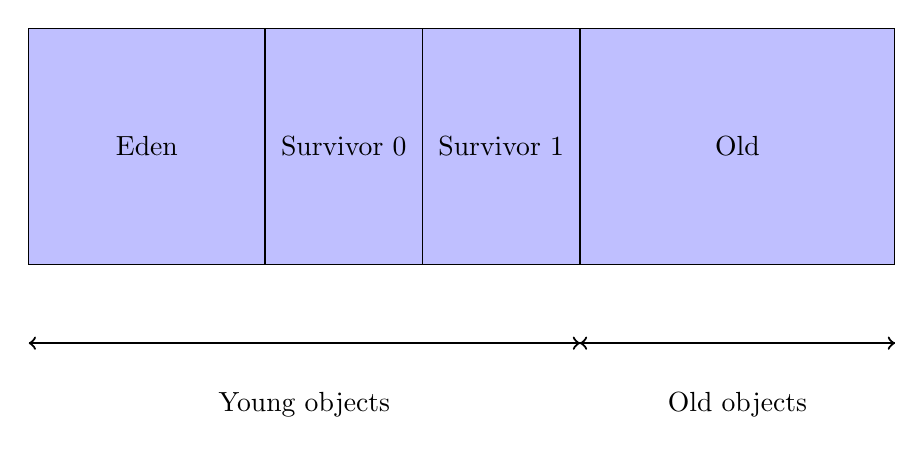
\begin{tikzpicture}
\node[yshift=-1.5cm, xshift=0cm, draw, rectangle, fill=blue!25, minimum width=3cm, minimum height=3cm] {Eden};
\node[yshift=-1.5cm, xshift=2.5cm, draw, rectangle, fill=blue!25, minimum width=2cm, minimum height=3cm] {Survivor 0};
\node[yshift=-1.5cm, xshift=4.5cm, draw, rectangle, fill=blue!25, minimum width=2cm, minimum height=3cm] {Survivor 1};
\node[yshift=-1.5cm, xshift=7.5cm, draw, rectangle, fill=blue!25, minimum width=4cm, minimum height=3cm] {Old};

\draw[thick, ->] (-1.5, -4) -- (5.5, -4);
\draw[thick, <-] (-1.5, -4) -- (5.5, -4);
\node[below] at(2, -4.5) {Young objects};

\draw[thick, ->] (5.5, -4) -- (9.5, -4);
\draw[thick, <-] (5.5, -4) -- (9.5, -4);
\node[below] at(7.5, -4.5) {Old objects};
\end{tikzpicture}

\end{frame}

\begin{frame}{Example of memory partition - JVM Heap 2}
	\begin{itemize}
		\item Eden space - When creating a new object memory is allocated from Eden space.
		\item Survivor space - Space of objects which survived garbage collection but have not reached tenuring threshold yet. Survivor space is divided into 2 equal spaces called "Survivor 0" and "Survivor 1".
		\item Old space - The objects to reach tenuring threshold are moved into Old space. Default value of tenuring threshold is 15 executions of garbage collector.
	\end{itemize}
\end{frame}

\end{document}
